% Chapter 5 - Desarrollo integral de una aplicación web usando la plataforma plusultra

\chapter{Desarrollo de una aplicaci\'{o}n web multimodal} % Chapter title

\label{ch:demo_development} 
% ### Introducción de capítulo
Los desarrollos de software en la web han avanzado desde sitios estáticos fuertemente orientados al hipertexto, en sus primeros años, a las \textit{aplicaciones} web actuales, similares en robustez y capacidad a las homólogas de escritorio pero con nuevas capacidades típicas del medio, como pueden ser aspectos de programación distribuida o tiempo real. Este avance no ha sido excluyente si no que se han ido añadiendo nuevas capas de funcionalidades. 

La aplicación web introducida en este capítulo tiene el objeto de actuar como herramienta de demostración y validación de la plataforma desarrollada, \emph{Plusultra}. Aunque también añade, a través de un conjunto de tecnologías, una nueva capa de funcionalidad multimodal al dominio de las aplicaciones web.

\section{Introducción} \label{sec:demo_intro}
Dentro del ámbito de una aplicación web, numerosos eventos pueden ocurrir, algunos generados por el usuario otros por la lógica de la aplicación (tanto cliente como servidor). Estos eventos generan en la mayoría de los casos que se dispare una acción y son usualmente acompañados por una animación a modo de feedback visual para darle fuerza al foco de la acción, ayudando a que el usuario mantenga en todo momento una ``imagen'' clara del estado del sistema, \ie~ que el usuario sepa qué ha ocurrido y que está ocurriendo. Pero esta no es la única forma de indicarle y/o darle mas feedback al usuario, existen diferentes vías de comunicación que pueden ser utilizadas con el simple e importante objetivo de brindar mas información y contexto \Eg~ un estado de error es comúnmente transmitido usando el color rojo; es posible agregar otro canal y estimular otro sensor, como puede ser la piel a través de una corta y clara vibración (similar a la que estamos recibimos de los smartphones), logrando así enriquecer la comunicación, cargando la autopista de información usuario-computador.

A través del uso de la plataforma \emph{plusultra} añadiremos un conjunto de nuevas modalidades al sistema, que generaran nuevos y definidos eventos para que puedan ser capturados dentro del ambiente de una aplicación web. Los usuarios de la misma se beneficiaran de estas nuevas capacidades de interacción, enriqueciendo así a una simple aplicación desarrollada a modo de probar las ventajas que provee el uso de la plataforma.

\subsection{Objetivo}
Desarrollar una aplicación web rica, utilizando un conjunto de dependencias acotado con el fin de hacer énfasis en el uso de la plataforma \emph{plusultra} y en el agregado de nuevas modalidades dentro de la aplicación.

La aplicación, si bien es de alcance limitado por ser una demostración, tiene el objeto de funcionar dentro del área de entretenimiento. Representa al clásico juego de niños de ``formas'', donde se busca estimular el reconocimiento y matcheo de patrones. Al hacer encajar las piezas en su lugar, se consigue una retroalimentación que puede verse incluso acompañado de estímulos externos (por parte de los padres, por ejemplo), premiando el éxito, es decir, esta acción de encastrar una pieza en su lugar; todo esto derivando en el conocimiento (y/o refuerzo) de nuevas formas para el niño.

Aquí se traslada este juego a una versión digital del mismo. A través del uso de la plataforma \emph{plusultra} y un conjunto acotado de modalidades, se extenderán las capacidades de interacción con el fin de generar mas estímulos en el usuario y así incrementar el \emph{feedback} total de la aplicación. 

\subsection{Requerimientos}
Mas allá de los requerimientos iniciales para desarrollar cualquier aplicación, la creación de una aplicación multimodal implica conocer cuáles son y cómo operan los dispositivos de modalidad que vayan a ser usados. 

Para el desarrollo puntual de esta aplicación fueron creados dos \emph{drivers} de modalidad para conectar dos nuevas modalidades, una háptica y otra aero-gestual. 
Estos controladores ofrecen un conjunto de eventos y en algunos casos abren un camino bi-direccional entre modalidad y aplicación, es decir, permiten la modificación de parámetros de modalidad en tiempo real. 

Mas adelante se muestran los principales detalles para la creación de un driver de modalidad genérico. 

\subsection{Módulos Principales}

A continuación se describen los principales módulos que componen a la aplicación \emph{shapes}:
\begin{itemize}
\item \texttt{main.js}; representa el contenedor principal de la aplicación, unifica las principales dependencias y dispara el inicio de la aplicación web junto con el panel visor de información de desarrollo.

\item \texttt{visor.js}; contiene la lógica necesaria para brindar información de estado útil para depurar la aplicación durante el desarrollo.

\item \texttt{shapes.js}; coordina los principales eventos de la aplicación, estos pueden ser eventos internos disparados por la aplicación o externos, despachados por alguna de las modalidades. Estos últimos, cuando ocurren son distribuidos a lo largo de todos los clientes conectados a la plataforma.

\item \texttt{interactive.js}; se encarga de administrar de manera uniforme los eventos de drag \& drop que ocurran en la aplicación.

\item \texttt{gyes.js}; es el módulo cliente oficial para conectarse con la plataforma \emph{plusultra}. Luego de obtener la llave de acceso a la plataforma, el desarrollador puede comenzar a utilizar un determinado número de instancias de la plataforma. El módulo brinda los principales eventos a los cuales la aplicación puede conectarse y actuar.

\item \texttt{HapticMD}; representa al controlador de modalidad háptico. El mismo esta desarrollado para aprovechar las capacidades de los dispositivos móviles modernos en el ámbito de una aplicación web rica. Provee eventos para definir interacción de entrada a través de gestos táctiles y de salida, a través de feedback vibro-táctiles.

\item \texttt{AirPointerMD}; es el controlador que administra la modalidad aero-gestual, \ie gestos aéreos, utilizando las manos. Este módulo utiliza como dispositivo de hardware al artefacto Leap, lo que permite conseguir información variada sobre manos y dedos sin necesidad de hardware extra \emph{en el} usuario. Este controlador brinda eventos de entrada sobre la posición de alguno de los dedos, el cual será usado como puntero para conseguir una manipulación básica directa sobre los elementos de la aplicación.
\end{itemize}

En la siguiente figura \ref{fig:demo_shapes_app}, se pueden observar a simple vista los principales módulos de la aplicación \emph{shapes}.
% FIGURA DE móduloS SHAPES APP
\begin{center}
  \begin{figure}[h]
    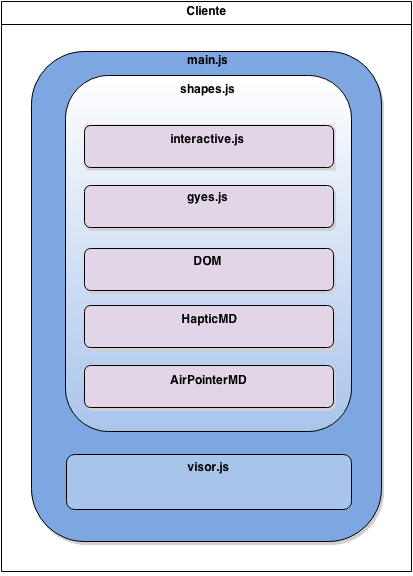
\includegraphics[scale=0.7]{gfx/shapes_app_demo}
    \caption{Módulos de la aplicación web Shapes}
    \label{fig:demo_shapes_app}
  \end{figure}
\end{center}


Los módulos desarrollados para esta aplicación se realizaron usando el patrón \emph{module}, como puede verse en \citet{demo:module_pattern}. A través del uso del mismo se consigue una división de responsabilidades y conocimiento, distinguiendo partes publicas (API) de privadas (implementación). Además permite aplicar una simple pero solida capacidad de manejo de dependencias internas. 

\subsection{Conectando a la Plataforma}
Con el fin de extender el conjunto de modalidades de una aplicación web, se propone la utilización de la plataforma \emph{plusultra}. La misma provee un servicio, en tiempo-real, de comunicación con dispositivos de modalidad. En el caso concreto de la aplicación \texttt{Shapes}, se han utilizado dos dispositivos de modalidad, el Leap Motion y los controladores táctiles de los dispositivos móviles. Agregar estas nuevas modalidades aumenta la capacidad de interacción con la aplicación desarrollada. Estas nuevas capacidades pueden ser aprovechadas por el desarrollador de la aplicación web mediante el consumo de los eventos que las mismas generan y que son transmitidos mediante la plataforma. 

En la figura \ref{fig:demo_shapes_app_arq} puede verse la relación entre los componentes arquitectonicos de la aplicación desarrollada:

% FIGURA DE ARQ SHAPES APP
\begin{center}
  \begin{figure}[h]
    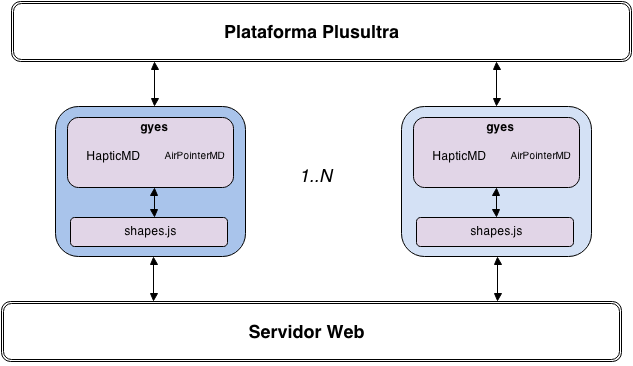
\includegraphics[scale=0.6]{gfx/shapes_app_arq}
    \caption{Vista de la arquitectura de la aplicación Shapes}
    \label{fig:demo_shapes_app_arq}
  \end{figure}
\end{center}


Para conectarse con la plataforma desde el contexto de una aplicación web el desarrollador debe incluir como una dependencia JavaScript, a su entorno de desarrollo, al módulo \texttt{gyes}. Este módulo brinda una interfaz de acceso a la plataforma.

Para conectarse es necesario contar con una llave de acceso y ejecutar el llamado a conexión usando el método \texttt{authenticate}. Este sistema de autenticación es simple y busca emular un escenario ``real''; debería ser mejorado acorde antes de ser llevado a un entorno de producción.

Luego de la autenticación el desarrollador puede comenzar a utilizar los drivers de modalidad que considere necesarios. Para esta aplicación se utilizan, un driver aero-gestual, denominado \emph{AirPointerMD} y otro, \emph{HapticMD}, usado como controlador háptico. A través del módulo \texttt{gyes} el desarrollador instancia las modalidades dentro de la aplicación web, por ejemplo:

\begin{lstlisting}
    // Construye una nueva modalidad háptica
    var hapticMod = new gyes.Modality( 'webHaptic', 'both', {} ); 
    // Configura algunas opciones del driver como por ej, qu\'{e} gestos hápticos capturar
    var driverOptions = {
      'hapticEvents': [ 'touch, hold' ],
      'element': doc.getElementById('shapes')
    };
    // Construye el driver de modalidad
    var hapticDriver = new HapticMD( driverOptions );
    // Conecta la modalidad con el driver
    hapticMod.use( hapticDriver );
    // Inserta la modalidad en la plataforma.
    _client.addModality( app_key, hapticMod );
\end{lstlisting}

Luego de instanciar y conectar las modalidades deben definirse las interpretaciones necesarias, \ie~ una estructura que da valor semántico a un conjunto de eventos (posiblemente generados por las modalidades) que ocurren en un intervalo de tiempo acotado. Entonces, para que una interpretación ocurra deben generarse determinados eventos en un instante de tiempo, la captura de estos eventos produce una fusión y es tratada por el motor de fusión distribuida del módulo \texttt{gyes}. Un ejemplo donde se muestra como instanciar el motor de fusión es el siguiente:

\begin{lstlisting}
    // El motor de fusión recibe interpretaciones como entrada.
    _gestureInterpretation = new gyes.Interpretation( ['fingerover', 'hold'] );
    // Algunas intepretaciones pueden producir sintetizado de eventos.
    _gestureInterpretation.canSynthetize( hapticMod.name, hapticDriver.getID(), 2000 );

    // Construcción de un motor de fusión.
    _fusion = new gyes.Fusion( {'verbose':true} );
    // Agregando interpretaciones al motor de fusión.
    _fusion.fuse( _gestureInterpretation );
\end{lstlisting}

Finalmente, luego de crear las interpretaciones necesarias junto al motor de fusión distribuida, lo único que queda por hacer es instanciar el sistema de fisión.

A través de este sistema, el desarrollador puede controlar programaticamente qué hacer cuando es detectada alguna interpretación. 

El sistema de fisión, permite conectar una función para que sea llamada de manera asincrónica luego de la ocurrencia de una interpretación, como puede verse a continuación:

\begin{lstlisting}
    // Construye el sistema de fisión
    var _fission = new gyes.Fission();
    
    // Conecta una interpretación con una función anónima.
    _fission.on( _gestureInterpretation.getName(), function(data){
      console.log( 'A new interpretation happened: ', data );
      gestName.textContent = '';
      gestElem.classList.remove( 'highlight' );
      gestDataText.classList.remove( 'invisible' );
      gestDataText.textContent = 'FISION';
      gestData.classList.add( 'highlight' );
      setTimeout(function(){
        gestDataText.classList.add( 'invisible' );
        gestData.classList.remove( 'highlight' );
        gestDataText.textContent = '';
      }, 2000);
    });
\end{lstlisting}

De esta forma se han mostrado los principales puntos de conexión necesarios para utilizar la plataforma \emph{plusultra} en su primera versión.

\section{Construcción de un Driver de Modalidad}
Para el desarrollo de una aplicación web multimodal es necesario contar con drivers o controladores que den soporte a los dispositivos de modalidad que vayan a ser usados. La plataforma \emph{plusultra} es agnóstica respecto al dispositivo de modalidad usado, brindando a través del módulo \emph{gyes} una interfaz para conectar un nuevo dispositivo al sistema. Un posible trabajo a futuro y aporte a la plataforma sería la creación de un catálogo online de todos los drivers de modalidad disponibles. 

El desarrollo de un nuevo driver de modalidad es una tarea relativamente simple, aunque esto puede variar entre dispositivos. El módulo \emph{gyes} provee una interfaz para la creación de drivers en JavaScript, aunque es posible desarrollar un driver en otro lenguaje, simplemente siguiendo el protocolo provisto por la plataforma \emph{plusultra}.
A continuación se muestran los principales métodos a implementar para crear un driver de modalidad, la conexión del mismo a la plataforma se definió anteriormente.

\begin{lstlisting}
// Incluir el canal de comunicación de gyes.
var ModalityDriverChannel = require( '../gyes/build/gyes' ).ModalityDriver;

// Declaramos el constructor del driver de modalidad. Ej:
module.exports = HapticModalityDriver;

// El constructor generado hereda los eventos a implementar del canal de drivers de modalidad.
inherits( HapticModalityDriver, ModalityDriverChannel );

// Si el dispositivo de modalidad puede sintetizar datos, entonces es posible conectar el evento de sintesis con alguna función interna. Ejemplo del driver háptico:
this.on( 'synthetized', this.fission.bind(this) );

// Si solo necesitamos disparar eventos de "entrada":
this.fire( 'recognized', {'gesture':data.type} );

\end{lstlisting}

Por lo tanto existen dos eventos importantes a tener en cuenta en la realización de un driver de modalidad; el evento para disparar algo ``sensado'' por el dispositivo, etiquetado como \emph{recognized} y el evento para recibir datos de parte de la aplicación y sintetizarlos, denominado \emph{synthetized}.
De esta forma es posible crear un nuevo driver para conectar un nuevo dispositivo al sistema y usarlo en el ámbito de una aplicación web. Es importante destacar que un componente creado de esta manera puede ser compartido y re-utilizado, la única dependencia es contar con el hardware indicado, es decir aquel para el cual fue desarrollado dicho driver. 

Esto permite pensar en la posibilidad de contar con un catalogo de drivers de la plataforma.

\section{Resumen del Capítulo}
El principal objetivo de la plataforma \emph{plusultra} es agrandar de manera uniforme el conjunto de modalidades que soportan actualmente las aplicaciones web. Este conjunto  es muy limitado, concentrado en las principales formas de comunicación con el ordenador, como lo son el mouse, el teclado y el feedback visual. En muy pocos casos una aplicación web va mas allá de eso y la principal razón puede estar ubicada en las dificultades propias de la tarea junto a la falta de información al respecto. Yendo un poco mas allá, imaginar el soporte a mas de una modalidad al mismo tiempo, parece difícil de visualizar y por ende de llevar a cabo.

Superar estas cuestiones fueron las premisas constantes durante el desarrollo de la plataforma y a través de la construcción de la aplicación ejemplo \texttt{Shapes} se mostró como es posible crear una aplicación web multimodal con un conjunto acotado y mínimo de  dependencias externas. Si bien existen cuestiones a mejorar, como la simplificación de la API del módulo \texttt{gyes} o las mejoras en el sistema de autenticación con la plataforma, la solución aquí propuesta ha funcionado como un recurso exitoso y concreto al problema de desarrollar una aplicación web multimodal.